\documentclass[12]{article}%12pt即为*四号字
\usepackage{ctex}%引入中文包
\usepackage{graphicx}%插入图片的包
\usepackage{geometry}%设置A4纸页边距的包
\usepackage{url}
\usepackage{stfloats}
\usepackage{float}
\geometry{left=3.18cm,right=3.18cm,top=2.54cm,bottom=2.54cm}%设置页边距
\linespread{1}%设置行间距



\begin{document}
\begin{center}
    \LARGE\songti\textbf{Chapter 3 homework} \\%标题
    \large\kaishu\textbf{褚朱钇恒\qquad 3200104144}%一般是我的姓名
\end{center}
    \section{Theoretical questions}
        \subsection{I}
            $s(1)=1,s^{'}(1)=3,s^{''}(1)=6$

            插值可得$p(x)=7x^3-18x^2+12x$,故$s^{''}(0)=-36\neq 0$

            故不是自然样条
        \subsection{II}
            \subsubsection{a}
                在每个区间上,f有三个待定系数,故共有$3(n-1)$个待定系数。

                在每个中间节点上,有$f_{i-1}=f_i,f^{'}_{i-1}=f^{'}_i$,引入两个条件。

                在每个形值点上,有$f_i=f(x_i)$,引入$n$个条件。

                故还需要确定$3(n-1)-2(n-2)-n=1$个条件。

            \subsubsection{b}
                在$x_i$处做泰勒展开得$p_i(x)=f_i+m_i(x-x_i)+a_i(x-x_i)^2$,将$p_i(x_{i+1})=f_{i+1}$,得

                $p_i(x)=f_i+m_i(x-x_i)+\frac{f_{i+1}-f_i-m_i(x_{i+1}-x_i)}{(x_{i+1}-x_i)^2}(x-x_i)^2$
            
            \subsubsection{c}
                根据(b)得,$m_{i+1}=-m_i+2\frac{f_{i+1}-f_i}{x_{i+1}-x_i}$,故可以递推求得$m_2,\cdots,m_{n-1}$

        \subsection{III}
            $s(0)=1+c,s^{'}(0)=3c,s^{''}(0)=6c$,故$s_2(x)=1+c+3cx+3cx^2+ax^3$

            由s为自然样条,$s^{''}(1)=6c+6a=0$,故$a=-c$,即$s_2(x)=1+c+3cx+3cx^2-cx^3$

            $s(1)=-1 \Rightarrow c=-\frac{1}{3}$

        \subsection{IV}
            \subsubsection{a}
                设$s_1(x)=a_1x^3+bx^2+cx+1$,$s_2(x)=a_2x^3+bx^2+cx+1$,

                由$f(-1)=f(1)=0,s^{''}(-1)=s^{''}(1)=0$,解得

                $s_1(x)=-\frac{1}{2}x^3-\frac{3}{2}x^2+1$
                ,$s_2(x)=\frac{1}{2}x^3-\frac{3}{2}x^2+1$
                
            \subsubsection{b}
                $\int_{-1}^{1}[s^{''}(x)]^2dx=6$

                (i)

                $g(x)=-x^2+1$

                $\int_{-1}^1[g^{''}(x)]^2dx=8 > \int_{-1}^{1}[s^{''}(x)]^2dx$

                (ii)

                $\int_{-1}^1[f^{''}(x)]^2dx=\frac{\pi^4}{16} \approx 6.08 > \int_{-1}^{1}[s^{''}(x)]^2dx$

        \subsection{V}
            \subsubsection{a}
            当$x\in[t_{i-1},t_i]$时,$B_i^2(x)=\frac{(x-t_{i-1})^2}{(t_{i+1}-t_{i-1})(t_{i}-t_{i-1})}$

            当$x\in[t_{i},t_{i+1}]$时,$B_i^2(x)=\frac{(x-t_{i-1})(t_{i+1}-x)}{(t_{i+1}-t_{i-1})(t_{i+1}-t_{i})}+\frac{(x-t_{i})(t_{i+2}-x)}{(t_{i+2}-t_{i})(t_{i+1}-t_{i})}$

            当$x\in[t_{i+1},t_{i+2}]$时,$B_i^2(x)=\frac{(x-t_{i+2})^2}{(t_{i+2}-t_{i})(t_{i+2}-t_{i+1})}$

            \subsubsection{b}
            $\frac{d}{dx}B^2_i(t_i^-)=\frac{2}{t_{i+1}-t_{i-1}}=\frac{d}{dx}B^2_i(t_i^+)$
            
            $\frac{d}{dx}B^2_i(t_{i+1}^-)=-\frac{2}{t_{i+2}-t_{i-1}}=\frac{d}{dx}B^2_i(t_{i+1}^+)$
            
            故$\frac{d}{dx}B^2_i$在$t_i$和$t_{i+1}$上连续。

            \subsubsection{c}
            当$x\in(t_{i-1},t_i)$时,$\frac{d}{dx}B^2_i=\frac{2(x-t_{i-1})}{(t_{i+1}-t_{i-1})(t_i-t_{i-1})}\neq 0$

            当$x\in(t_{i},t_{i+1})$时,$\frac{d}{dx}B^2_i$为线性函数,故只有一处$x^*$为0.

            $x^*=\frac{(t_{i+1}+t_{i-1})(t_{i+2}-t_{i})+(t_{i+2}+t_{i})(t_{i+1}-t_{i-1})}{2(t_{i+1}+t_{i+2}-t_{i-1}-t_{i})}$

            \subsubsection{d}
            只需考虑边界点和极值点,$B_i^2(t_i)=0$,$B_i^2(x^*)< 1$

            故$B^2_i(x)\in [0,1)$
            \subsubsection{e}
            \begin{figure}[H]
                \centering
                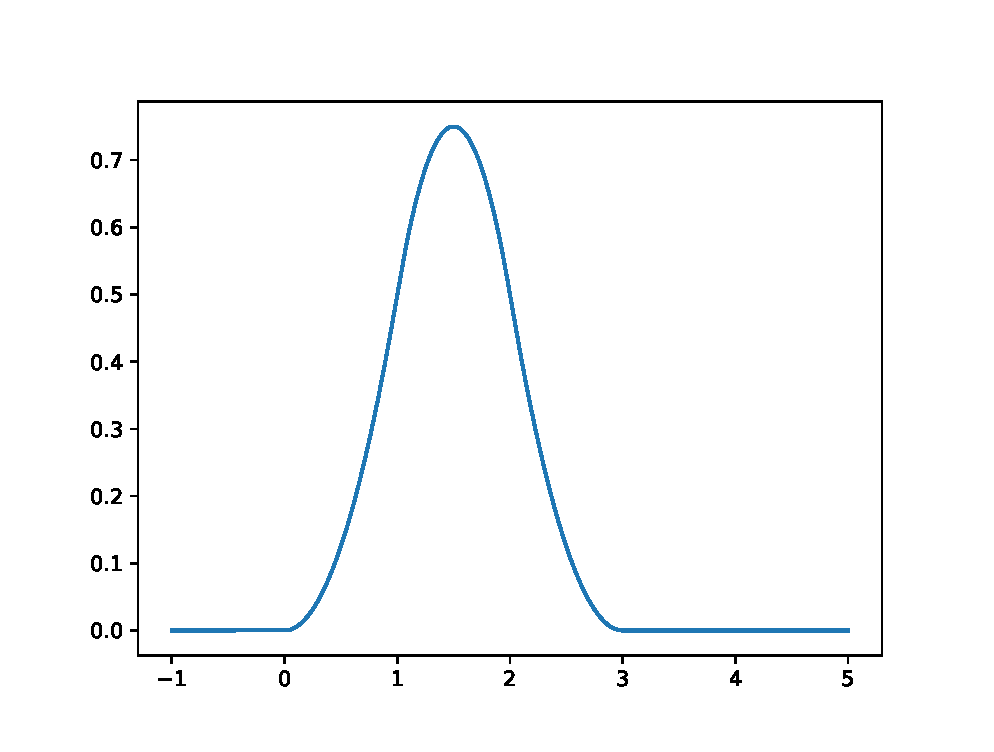
\includegraphics[width=0.7\textwidth]{./pic/e.eps}
                \caption{$B_1^2(x)$的图像}
            \end{figure}

        \subsection{VI}
        $LHS=[t_i,t_{i+1},t_{i+2}](t-x)^2_+-[t_{i-1},t_{i},t_{i+1}](t-x)^2_+$

        当$x\le t_{i-1}$时,$LHS=0=RHS$

        当$t_{i-1}<x\le t_{i}$时,$LHS=\frac{(x-t_{i-1})^2}{(t_{i+1}-t_{i-1})(t_{i}-t_{i-1})}=RHS$

        当$t_i<x\le t_{i+1}$时,$LHS=\frac{(x-t_{i-1})(t_{i+1}-x)}{(t_{i+1}-t_{i-1})(t_{i+1}-t_{i})}+\frac{(x-t_{i})(t_{i+2}-x)}{(t_{i+2}-t_{i})(t_{i+1}-t_{i})}=RHS$

        当$t_{i+1}<x\le t_{i+2}$时,$LHS=\frac{(x-t_{i+2})^2}{(t_{i+2}-t_{i})(t_{i+2}-t_{i+1})}=RHS$

        当$x> t_{i+2}$时,$LHS=0=RHS$

        综上,原等式成立。
            

        \subsection{VII}
            由B样条的微分性质,$\frac{d}{dx}B_i^n(x)=\frac{nB^{n-1}_i(x)}{t_{i+n-1}-t_{i-1}}-\frac{nB^{n-1}_{i+1}(x)}{t_{i+n}-t_{i}}$

            那么有$\int_{t_{i-1}}^{t_{i+n}}\frac{B^n_i(x)}{t_{i+n}-t_{i-1}}dx-\int_{t_{i}}^{t_{i+n+1}}\frac{B^n_{i+1}(x)}{t_{i+n+1}-t_{i}}dx=$

            $\int_{t_{i-1}}^{t_{i+n+1}}[\frac{B^n_i(x)}{t_{i+n}-t_{i-1}}-\frac{B^n_{i+1}(x)}{t_{i+n+1}-t_{i}}]dx=$
            
            $\frac{1}{n}B^{n+1}_i(x)|_{t_{i-1}}^{t_{i+n+1}}=0$ 
            
            故$\int_{t_{i-1}}^{t_{i+n}}\frac{B^n_i(x)}{t_{i+n}-t_{i-1}}dx=\int_{t_{i}}^{t_{i+n+1}}\frac{B^n_{i+1}(x)}{t_{i+n+1}-t_{i}}dx$,原命题成立
        \subsection{VIII}
            该命题可表示为$\forall m \in N ,\forall n=0,1,\cdots m$

            $\tau_{m-n}(x_0,\cdots,x_n)=[x_0,\cdots,x_n]x_m$

            (a)当$m=4,n=2$时,可列出差商表

            \begin{tabular}{c|c|c|c}
                $x_1 $& $x_1^4$  \\
                $x_2$ & $x_2^4$  & $x_1^3+x_1^2x_2+x_1x_2^2+x_2^3$ \\
                $x_3$ & $x_3^4$  & $x_2^3+x_2^2x_3+x_2x_3^2+x_3^3$ & $x_1^2+x_2^2+x_3^2+x_1x_2+x_2x_3+x_1x_3$ \\
            \end{tabular}

            故有$\tau_{2}(x_1,x_2,x_3)=[x_1,x_2,x_3]x^4$

            (b)

            由$(x_{n+1}-x_0)\tau_k(x_0,\cdots,x_n,x_{n+1})$

            $=\tau_{k+1}(x_0,\cdots,x_n,x_{n+1})-\tau_{k+1}(x_0,\cdots,x_n)-x_0\tau_k(x_0,\cdots,x_n,x_{n+1})$

            $=\tau_{k+1}(x_1,\cdots,x_n,x_{n+1})-\tau_{k+1}(x_0,\cdots,x_n)$

            当$n=0$时,$\forall m$,有$\tau_m(x_0)=[x_0]x^m$.

            假设对某个$n<m$,原式成立,则有

            $\tau_{m-n-1}(x_0,\cdots,x_{n+1})$

            $=\frac{\tau_{m-n}(x_1,\cdots,x_n,x_{n+1})-\tau_{m-n}(x_0,\cdots,x_n)}{x_{n+1}-x_0}$
            
            $=\frac{[x_1,\cdots,x_n,x_{n+1}]x^m-[x_0,\cdots,x_n]x^m}{x_{n+1}-x_0}$

            $=[x_0,\cdots,x_n,x_{n+1}]x^m$

            故原命题成立。
            
\end{document} 